\documentclass[12pt,a4paper]{article}
\usepackage[UTF8]{ctex}
\usepackage{geometry}
\geometry{a4paper,left=2.5cm,right=2.5cm,top=2.5cm,bottom=2.5cm}

% 基础宏包
\usepackage{amsmath}           % 数学公式
\usepackage{amssymb}          % 数学符号
\usepackage{graphicx}          % 图片支持
\usepackage{float}             % 浮动体设置
\usepackage{booktabs}          % 用于美观的表格边框
\usepackage{fancyhdr}          % 页眉页脚
\usepackage{lastpage}          % 获取总页数
\usepackage{zhnumber}          % 中文数字
\usepackage{subcaption}        % 支持子图
\usepackage{placeins}          % 用于\FloatBarrier命令

% 参考文献设置
\usepackage[numbers,sort&compress,square,comma]{natbib}
\bibliographystyle{unsrtnat}

% URL和超链接设置
\usepackage{url}
\usepackage{xurl}
\usepackage{hyperref}
\renewcommand{\UrlFont}{\ttfamily\color{blue}\small}

% 浮动体设置
\renewcommand{\textfraction}{0.05}
\renewcommand{\topfraction}{0.9}
\renewcommand{\bottomfraction}{0.9}
\renewcommand{\floatpagefraction}{0.8}
\setcounter{topnumber}{3}
\setcounter{bottomnumber}{3}
\setcounter{totalnumber}{5}

% 引入样式文件
% 基础包引用
\usepackage{amsmath}
\usepackage{graphicx}
\usepackage{float}
\usepackage{setspace}
\usepackage{xargs}
\usepackage{nameref}
\usepackage{appendix}
\usepackage{cite}
\usepackage{hyperref}
\usepackage{fancyref}
\usepackage{scrextend}

% 颜色定义
\usepackage[dvipsnames]{xcolor}
\definecolor{cleanOrange}{HTML}{D14D00}
\definecolor{cleanYellow}{HTML}{FFFF99}
\definecolor{cleanBlue}{HTML}{3d0099}

% 通用命令
\newcommand\tab[1][1cm]{\hspace*{#1}}
\hypersetup{colorlinks=true, linkcolor=black}
\interfootnotelinepenalty=10000

% 注释和标记
\usepackage[colorinlistoftodos,prependcaption,textsize=footnotesize]{todonotes}
\newcommandx{\commred}[2][1=]{\textcolor{Red}{\todo[linecolor=red,backgroundcolor=red!25,bordercolor=red,#1]{#2}}}
\newcommandx{\commblue}[2][1=]{\textcolor{Blue}{\todo[linecolor=blue,backgroundcolor=blue!25,bordercolor=blue,#1]{#2}}}
\newcommandx{\commgreen}[2][1=]{\textcolor{OliveGreen}{\todo[linecolor=OliveGreen,backgroundcolor=OliveGreen!25,bordercolor=OliveGreen,#1]{#2}}}
\newcommandx{\commpurp}[2][1=]{\textcolor{Plum}{\todo[linecolor=Plum,backgroundcolor=Plum!25,bordercolor=Plum,#1]{#2}}}

% 代码和注释
\def\code#1{{\tt #1}}
\def\note#1{\noindent{\bf [Note: #1]}}

% 附录格式
\makeatletter
\def\@seccntformat#1{\@ifundefined{#1@cntformat}%
   {\csname the#1\endcsname\quad}%
   {\csname #1@cntformat\endcsname}%
}
\let\oldappendix\appendix
\renewcommand\appendix{%
    \oldappendix
    \newcommand{\section@cntformat}{\appendixname~\thesection\quad}
}
\makeatother 
% 页面布局设置
\usepackage{geometry}
\geometry{a4paper,left=2.3cm,right=2.3cm,top=2.7cm,bottom=2.7cm}

% 页眉页脚
\usepackage{fancyhdr}
\usepackage{lastpage}
\pagestyle{fancy}
\renewcommand{\headrulewidth}{0.1pt}
\renewcommand{\footrulewidth}{0pt}

% 章节格式
\usepackage{sectsty}
\sectionfont{\LARGE}
\subsectionfont{\Large}
\subsubsectionfont{\large}

% 表格设置
\usepackage{tabularx}
\usepackage{booktabs}
\usepackage{multirow}
\usepackage{array}  % 提供高级表格功能
\usepackage{makecell} % 用于表格单元格中的换行
\usepackage{threeparttable} % 为表格添加注释

% 表格间距设置
\setlength{\tabcolsep}{5pt} % 列间距
\renewcommand{\arraystretch}{1.2} % 行间距

% 定义新的列类型,用于居中显示文本
\newcolumntype{C}[1]{>{\centering\arraybackslash}p{#1}}
\newcolumntype{L}[1]{>{\raggedright\arraybackslash}p{#1}}
\newcolumntype{R}[1]{>{\raggedleft\arraybackslash}p{#1}}

% 图表设置
\usepackage{caption}
% \usepackage{subfigure} % 已在main.tex中使用subcaption代替
\setlength{\textfloatsep}{10mm}

% 标题线设置
\providecommand{\HRule}{\rule{\linewidth}{0.5mm}}
\providecommand{\HRulegrossa}{\rule{\linewidth}{1.2mm}} 
% 字体和编码设置
\usepackage{ctex}
\usepackage[utf8]{inputenc}
\usepackage[british,UKenglish]{babel}

% 字体命令
\newcommand{\cleancode}[1]{\begin{addmargin}[3em]{3em}\texttt{\textcolor{cleanOrange}{#1}}\end{addmargin}}
\newcommand{\cleanstyle}[1]{\text{\textcolor{cleanOrange}{\texttt{#1}}}} 
% 代码样式设置
\usepackage[T1]{fontenc}
\usepackage[scaled=0.82]{beramono}
\usepackage{microtype}
\usepackage[procnames]{listings}

% 代码颜色定义
\definecolor{dkgreen}{rgb}{0,0.6,0}
\definecolor{gray}{rgb}{0.5,0.5,0.5}
\definecolor{mauve}{rgb}{0.58,0,0.82}

% 基础代码样式
\lstset{
  frame=tb,
  aboveskip=3mm,
  belowskip=3mm,
  showstringspaces=false,
  columns=fixed,
  basicstyle={\small\ttfamily},
  numbers=left,
  numberstyle=\tiny\color{gray},
  keywordstyle=\color{blue},
  commentstyle=\color{dkgreen},
  stringstyle=\color{mauve},
  frame=single,
  breaklines=true,
  breakatwhitespace=true,
  tabsize=2
}

% Scala语言定义
\lstdefinelanguage{scala}{
  morekeywords={abstract,case,catch,class,def,
    do,else,extends,false,final,finally,
    for,if,implicit,import,match,mixin,
    new,null,object,override,package,
    private,protected,requires,return,sealed,
    super,this,throw,trait,true,try,
    type,val,var,while,with,yield},
  sensitive=true,
  morecomment=[l]{//},
  morecomment=[n]{/*}{*/},
  morestring=[b]",
  morestring=[b]',
  morestring=[b]"""
}

% 语言环境定义
\lstnewenvironment{scala}[1][]
{\lstset{language=scala,#1}}
{}
\lstnewenvironment{cpp}[1][]
{\lstset{language=C++,#1}}
{}
\lstnewenvironment{bash}[1][]
{\lstset{language=bash,#1}}
{}
\lstnewenvironment{verilog}[1][]
{\lstset{language=verilog,#1}}
{} 

% 图片路径
\graphicspath{{fig/}}

% 设置中文段首缩进
\setlength{\parindent}{2em}  % 段首缩进2个字符
\setlength{\parskip}{0.5ex}  % 段间距

% 确保文献内含中文字符时正确编译
\usepackage{etoolbox}
\patchcmd{\thebibliography}{\sloppy}{\sloppy\raggedright}{}{}

% 自定义参考文献样式
\makeatletter
\renewcommand{\@biblabel}[1]{[#1]}
\def\@cite#1#2{[#1\if@tempswa, #2\fi]}
\renewcommand{\bibfont}{\small}
\setlength{\bibsep}{1.2ex}
\makeatother

% 伪代码设置
\usepackage{algorithm}  
\usepackage{algorithmicx}  
\usepackage{algpseudocode}  
\floatname{algorithm}{Algorithm}  
\renewcommand{\algorithmicrequire}{\textbf{Input:}}  
\renewcommand{\algorithmicensure}{\textbf{Output:}} 
\usepackage{lipsum}  

% 定义中英文摘要环境
\makeatletter
% 中文摘要环境
\newenvironment{cnabstract}{
    \par\small
    \noindent\mbox{}\par\vspace{-\baselineskip}
    \par\songti\parindent 2em
    }
    {\par\vspace{1em}}

% 英文摘要环境
\newenvironment{enabstract}{
    \par\small
    \noindent\mbox{}\par\vspace{-\baselineskip}
    \par\parindent 2em
    }
    {\par\vspace{1em}}
\makeatother

\makeatletter
\providecommand{\breakablealgorithm}{%
  \begin{center}
     \refstepcounter{algorithm}%
     \hrule height.8pt depth0pt \kern2pt%
     \renewcommand{\caption}[2][\relax]{%
      {\raggedright\textbf{\ALG@name~\thealgorithm} ##2\par}%
      \ifx\relax##1\relax
         \addcontentsline{loa}{algorithm}{\protect\numberline{\thealgorithm}##2}%
      \else
         \addcontentsline{loa}{algorithm}{\protect\numberline{\thealgorithm}##1}%
      \fi
      \kern2pt\hrule\kern2pt
     }
  \end{center}
}
\makeatother

%-------------------------页眉页脚--------------
\pagestyle{fancy}
\lhead{\kaishu \leftmark}
\rhead{\kaishu 预测驱动统计推断:一项模拟研究}
\lfoot{}
\cfoot{\thepage}
\rfoot{}

%--------------------文档内容--------------------

\begin{document}
\renewcommand{\contentsname}{目录}
\renewcommand{\appendixname}{附录}
\renewcommand{\appendixpagename}{附录}
\renewcommand{\refname}{参考文献} 
\renewcommand{\figurename}{图}
\renewcommand{\tablename}{表}
\renewcommand{\abstractname}{摘要}
\renewcommand{\today}{\number\year 年 \number\month 月 \number\day 日}

\renewcommand {\thefigure}{\thesection{}.\arabic{figure}}%图片按章标号
\renewcommand{\figurename}{图}
\renewcommand{\contentsname}{目录}  
\cfoot{\thepage\ of \pageref{LastPage}}%当前页 of 总页数

% 封面
\begin{titlepage}
    \begin{center}
    
\includegraphics[width=0.6\textwidth]{NKU.png}\\[1cm]
    \vspace{20mm}
		\textbf{\huge\textbf{\kaishu{数据科学导论实验报告}}}\\[0.5cm]
		\textbf{\huge{\kaishu{预测驱动统计推断:一项模拟研究}}}\\[2.3cm]

		\vspace{\fill}
    
    \centering
    \textsc{\LARGE \kaishu{徐媛}}\\[0.5cm]
    \textsc{\LARGE \kaishu{学号\ :\ 2313072}}\\[0.5cm]
    \textsc{\LARGE \kaishu{徐凡舒}}\\[0.5cm]
    \textsc{\LARGE \kaishu{学号\ :\ 2312754}}\\[0.5cm]
    \textsc{\LARGE \kaishu{谢筱昀}}\\[0.5cm]
    \textsc{\LARGE \kaishu{学号\ :\ 2310726}}\\[0.5cm]
    \vfill
    {\Large \today}
    \end{center}
\end{titlepage}

% --- Chinese Abstract ---
\clearpage
\phantomsection % For correct hyperlinking
\addcontentsline{toc}{section}{摘要}
\begin{center}
    {\zihao{3}\songti\bfseries 摘\quad 要}
\end{center}
\vspace{0.5em}
\small
\setlength{\parindent}{2em} % Standard Chinese paragraph indent

\indent 本项目旨在评估预测驱动推断(Prediction-Powered Inference, PPI)框架在结合少量标注数据、大量未标注数据及机器学习模型预测以提升统计推断效率方面的性能。通过模拟一个类似阿尔茨海默病神经影像学倡议(ADNI)的数据集,我们比较了PPI方法与经典统计推断(仅依赖少量标注数据)和朴素机器学习推断(直接使用所有预测值)的表现。实验结果表明,PPI方法能够在保持名义覆盖率的同时,有效缩小置信区间宽度,并显著降低估计偏差,从而验证了其在数据稀缺场景下增强统计推断能力的潜力。代码已开源于 \url{https://github.com/aokimi0/ppl}。

\vspace{1em}
\noindent\textbf{关键词:}预测驱动推断;统计推断;机器学习;数据稀缺;模拟研究;置信区间

% --- English Abstract ---
\clearpage
\phantomsection
\addcontentsline{toc}{section}{Abstract}
\begin{center}
    {\zihao{3}\bfseries Abstract}
\end{center}
\vspace{0.5em}
\small
\setlength{\parindent}{2em}

\indent This project aims to evaluate the performance of the Prediction-Powered Inference (PPI) framework in enhancing statistical inference efficiency by combining a small amount of labeled data, a large amount of unlabeled data, and predictions from machine learning models. By simulating a dataset analogous to the Alzheimer's Disease Neuroimaging Initiative (ADNI), we compare the PPI method with classical statistical inference (relying solely on limited labeled data) and naive machine learning inference (directly using all predicted values). The experimental results demonstrate that the PPI method can effectively reduce confidence interval width and significantly decrease estimation bias while maintaining nominal coverage rates, thereby validating its potential to enhance statistical inference capabilities in data-scarce scenarios. The code is available at \url{https://github.com/aokimi0/ppl}.

\vspace{1em}
\noindent\textbf{Keywords:} Prediction-Powered Inference; Statistical Inference; Machine Learning; Data Scarcity; Simulation Study; Confidence Intervals

% --- Table of Contents ---
\clearpage
\tableofcontents
\clearpage

% --- Main Content Start ---
\section{引言}
\subsection{背景与动机}
\indent 在许多科学研究和商业决策中,获取大规模高质量的标注数据("金标准")成本高昂且耗时。然而,未标注数据和强大的预训练机器学习模型却日益普及。传统的统计推断方法在标注数据稀缺时面临统计功效不足的问题,而直接将机器学习模型的预测结果用于下游统计分析,则可能因模型偏差导致推断失效。预测驱动推断(PPI)框架的提出,旨在弥合机器学习预测能力与统计推断有效性要求之间的鸿沟。

\subsection{问题陈述}
\indent 本项目探讨的核心问题是:当拥有少量标注数据、大量未标注数据以及一个(可能不完美的)机器学习预测模型时,如何有效地结合这些信息进行可靠的统计推断(如均值估计和置信区间构建)?我们旨在量化PPI方法相对于仅使用标注数据的经典方法和直接使用模型预测的朴素方法的性能增益。

\subsection{项目目标}
\begin{enumerate}
    \item 实现一个基础的PPI框架用于总体均值的估计。
    \item 生成一个模拟的医学数据集,以模拟真实世界中数据稀缺和模型不完美的场景。
    \item 比较PPI方法、经典统计方法和朴素ML方法在估计偏差、置信区间宽度和覆盖率方面的表现。
    \item 通过可视化展示不同方法的性能差异。
    \item 撰写实验报告,总结研究发现。
\end{enumerate}

\subsection{范围与贡献}
\label{sec:scope_contribution}
本项目将聚焦于特定类型的统计推断任务,例如总体均值的估计、总体分位数的估计,或线性回归模型中特定系数的估计,并为这些估计量构建置信区间。所选用的核心方法将是预测驱动推断(Prediction-Powered Inference, PPI)框架的一个变体,很可能是PPI++,因为它在效率和自适应性方面具有优势。

本项目的贡献在于提供一个在常见数据科学场景下(即标注数据稀缺但存在未标注数据和预训练模型)应用和评估预测驱动推断方法的实用指南和实证研究。通过清晰展示其相对于传统方法和朴素ML预测应用的优势,本项目旨在为数据科学从业者和研究者提供一种更可靠、更高效地利用现有数据资源进行统计推断的思路和工具。

\subsection{报告结构}
\label{sec:report_structure}
本报告的后续章节安排如下:第二部分将详细介绍预测驱动统计推断的理论框架,包括其基本原理、核心组件(如校正项)以及所选PPI++方法的特点。第三部分将阐述实验设计和具体实现细节,包括数据集的选择与预处理、预训练模型的规格、三种对比推断方法的实现方案,以及开发环境和所用工具。第四部分将呈现实验结果和评估,重点比较不同方法在点估计偏差、均方误差、置信区间覆盖率和长度等方面的表现。第五部分将对实验结果进行深入讨论,解读其含义,分析研究的局限性,并展望未来工作。第六部分为结论,总结本研究的主要发现和意义。最后是参考文献和附录。

\section{方法论}
\label{sec:methodology}

\subsection{预测驱动的统计推断框架}
\label{sec:ppi_framework}
\indent 在现代数据科学实践中,一个核心的挑战在于如何弥合机器学习强大的预测能力与经典统计学对推断结论严格有效性要求之间的鸿沟。机器学习模型,特别是大规模预训练模型,能够从未标注数据中学习并生成海量的预测信息,但这些预测本身并不直接提供统计学意义上的不确定性量化。另一方面,传统的统计推断方法虽然能提供严格的有效性保证(如置信区间的正确覆盖率),但在标注数据稀缺时其效能大打折扣。预测驱动推断(PPI)及其变体,正是为了解决这一核心矛盾而提出的。它们不试图替代统计推断,而是旨在将机器学习的预测信息以一种统计学上稳健的方式整合到推断过程中,从而在保证有效性的前提下,提升推断的效率和精度。这一框架的一个显著优点在于其对机器学习模型的"不可知论(agnosticism)": 它不要求深入了解预训练模型的内部结构或训练细节,仅利用其输出的预测值,并通过少量标注数据来校正这些预测中可能存在的系统性偏差。这种特性使得PPI方法具有广泛的适用性,尤其是在用户可能无法控制或完全理解所用预训练模型的场景中。

\subsubsection{预测驱动推断(PPI)基础}
\label{sec:ppi_basics}
\indent 预测驱动推断(Prediction-Powered Inference, PPI)是一种新兴的统计框架,其核心思想在于巧妙地结合两类数据源的优势:一类是数量庞大但可能存在未知偏差的机器学习(ML)模型预测结果,另一类是数量稀少但质量可靠的"金标准"标注数据。PPI的目标是利用这两类信息,对感兴趣的总体参数(如均值、分位数、回归系数等)进行有效的统计推断,即构建具有预设覆盖率的置信区间或进行假设检验。

该框架的一般流程是:首先,利用预训练的ML模型 $f(X)$ 对大量的未标注数据 $X'_1, \dots, X'_N$ 产生预测值 $\hat{Y}'_1, \dots, \hat{Y}'_N$。这些预测值被用来形成对目标参数的一个初步的、可能是有偏的估计。然后,利用小规模的标注数据集 $(X_1,Y_1), \dots, (X_n,Y_n)$,其中 $Y_i$ 是真实的标签,而 $\hat{Y}_i=f(X_i)$ 是ML模型对这些已标注样本的预测。通过比较 $Y_i$ 和 $\hat{Y}_i$,PPI能够量化ML模型的预测误差,并构建一个所谓的"校正项"(rectifier)。这个校正项随后被用来调整基于大量预测值得出的初步估计,从而得到一个经过偏差校正的、更可靠的最终估计量。

PPI框架的普适性很强,它可以应用于任何能够表示为凸目标函数最小化器的参数估计问题。这意味着除了常见的均值、分位数和回归系数外,许多其他复杂的统计量也可以通过PPI进行推断。一个关键特性是,PPI对提供预测的ML模型 $f(X)$ 本身不作任何假设,无论是模型的结构、训练方法还是其预测的准确度如何,PPI都能保证最终推断的统计有效性。

\subsubsection{校正项(Rectifier)在偏差修正中的作用}
\label{sec:rectifier}
校正项是PPI框架中实现偏差修正的核心机制。其基本思想是利用已有的少量标注数据来估计和补偿由ML模型预测引入的系统性偏差。校正项的具体数学形式取决于所要估计的目标参数 $\theta$ 以及相应的"拟合度量"(measure of fit) $m_{\theta}$。

在Angelopoulos等人的原始工作中,对于一个候选的参数值 $\theta$,拟合度量 $m_{\theta}$ 在基于预测值 $\hat{Y}'$ 的未标注数据集上计算,用于量化 $\theta$ 基于这些(可能不完美的)预测数据的合理性。校正项 $D_{\theta}$ (或 $\Delta_{\theta}$) 则被定义为在标注数据集上,真实标签 $Y$ 计算的拟合度量与预测标签 $\hat{Y}$ 计算的拟合度量之差。例如,在估计总体均值 $\mu=E[Y]$ 的简单情况下,一个朴素的基于预测的估计是 $\frac{1}{N}\sum_{i=1}^{N}f(X'_i)$。校正项可以理解为对 $f(X)$ 预测偏差的经验估计,通常形式为 $\frac{1}{n}\sum_{j=1}^{n}(f(X_j)-Y_j)$,即模型预测值与真实值在标注样本上的平均差异。

最终的PPI估计量 $\hat{\theta}_{\text{PPI}}$ 通常是将基于大量预测的初步估计量减去这个校正项(或其某种形式的推广)得到。例如,对于均值估计,PPI估计量可以表示为:
\begin{equation}
\hat{\mu}_{\text{PPI}} = \frac{1}{N} \sum_{i=1}^{N} f(X'_i) - \frac{1}{n} \sum_{j=1}^{n} (f(X_j) - Y_j)
\label{eq:ppi_estimator_new}
\end{equation}
这个校正步骤确保了 $\hat{\theta}_{\text{PPI}}$ (在此例中为 $\hat{\mu}_{\text{PPI}}$)是目标参数 $\theta$ 的一个(渐进)无偏估计量。通过这种方式,即使ML模型的预测 $f(X)$ 存在系统性偏差,只要这个偏差能够在标注数据上被稳定地估计出来,PPI就能够有效地消除它对最终统计推断的影响,从而保证置信区间的有效覆盖率和假设检验的I类错误控制。

\subsubsection{所选PPI变体:PPI++ 以增强效率和自适应性}
\label{sec:ppi_plus_plus}
尽管原始PPI框架具有开创性和普适性,但在某些情况下,其计算效率和统计效率可能并非最优。为了解决这些问题,Angelopoulos等人后续提出了PPI++。PPI++ 的核心改进在于引入了一个称为"功效调整参数"(power-tuning parameter)的 $\lambda \in \mathbb{R}$。这个参数用于自适应地权衡经典统计估计量(仅基于标注数据)和利用ML预测进行校正的部分。

PPI++的估计量通常基于一个调整后的损失函数 $L^{\text{PP}}_{\lambda}(\theta)$,其形式为:
\begin{equation}
L^{\text{PP}}_{\lambda}(\theta) := L_n(\theta) + \lambda \cdot (L_f^N(\theta) - L_f^n(\theta))
\label{eq:ppi_plus_plus_loss}
\end{equation}
其中,$L_n(\theta)$ 是基于标注数据的经典损失函数,$L_f^N(\theta)$ 是基于大量未标注数据(使用 $f(X)$ 的预测值)的损失函数,$L_f^n(\theta)$ 是基于标注数据(但使用 $f(X)$ 的预测值而非真实 $Y$)的损失函数。参数 $\lambda$ 控制了预测信息(即 $L_f^N(\theta) - L_f^n(\theta)$ 这一项,它反映了预测在未标注数据上带来的"增益"相对于其在标注数据上的"表现")在多大程度上被纳入最终估计。

$\lambda$ 的选择至关重要。PPI++的一个关键特性是,$\lambda$ 可以从数据中估计得到,目标通常是最小化最终PPI++估计量的渐进方差或最大化相关假设检验的功效。Python库 \texttt{ppi\_py} 在其实现中,允许用户不指定 \texttt{lam} 参数,此时库会自动从数据中估计最优的 $\lambda$ 值。当 $\lambda=0$ 时,PPI++估计量退化为仅使用标注数据的经典估计量;当 $\lambda=1$ 时,在某些特定情况下(例如,损失函数具有特定形式),PPI++可能恢复到原始PPI估计量的形式。

这种自适应性是PPI++相较于原始PPI的一个重要优势。它使得方法能够根据预训练模型 $f(X)$ 的实际预测质量自动调整。如果 $f(X)$ 的预测非常准确,估计出的 $\lambda$ 可能会接近1,从而充分利用大量的预测信息以减小估计方差、缩短置信区间。反之,如果 $f(X)$ 的预测质量较差或与真实值关联不大,估计出的 $\lambda$ 可能会趋向于0,此时PPI++将更多地依赖于可靠的标注数据,表现接近于经典推断方法,从而避免了被劣质预测误导的风险。这种稳健性使得PPI++在实际应用中更具吸引力,因为它确保了(在渐进意义下)其表现至少不劣于仅使用标注数据的经典方法,并且在预测信息有用时能显著提升推断效率。

\subsubsection{与预训练模型 $f(X)$ 的集成}
\label{sec:integration_with_fX}
PPI/PPI++框架与预训练模型 $f(X)$ 的集成方式非常直接且灵活。预训练模型 $f(X)$ 的角色是为特征向量 $X$ 提供预测值 $\hat{Y}$。这些预测值将在两个关键环节被使用:
\begin{enumerate}
    \item \textbf{在标注数据集上}:对于每一个标注样本 $(X_j,Y_j)$,模型会产生预测 $\hat{Y}_j=f(X_j)$。这些预测值 $\hat{Y}_j$ 与真实标签 $Y_j$ 一同用于计算校正项,如前文所述。
    \item \textbf{在大量未标注数据集上}:对于每一个未标注样本 $X'_i$,模型会产生预测 $\hat{Y}'_i=f(X'_i)$。这些预测值 $\hat{Y}'_i$ 被用来构建对目标参数的初步估计,该估计随后会被校正项调整。
\end{enumerate}
PPI/PPI++框架的一个核心优势在于其对预训练模型 $f(X)$ 的"黑箱"处理方式。这意味着研究者无需关心 $f(X)$ 的具体架构(例如,是线性模型、决策树、神经网络还是更复杂的集成模型)、训练细节(例如,训练数据、优化算法、超参数设置)或其内部工作原理。只要模型能够输入特征 $X$ 并输出对目标变量 $Y$ 的预测 $\hat{Y}$,它就可以被整合到PPI框架中。这种模型无关性极大地增强了PPI方法的实用性和普适性,使得研究者可以方便地利用已有的、可能是由第三方提供的、或者结构非常复杂的预训练模型,而无需对其进行修改或深入分析。

\subsubsection{处理潜在的分布偏移(简述)}
\label{sec:distribution_shift}
\indent 在实际应用中,标注数据和未标注数据的来源或收集条件可能存在差异,导致它们的概率分布不完全一致,即存在分布偏移(distribution shift)。PPI框架及其变体也考虑了这类更具挑战性的情况,并提供相应的解决方案,以保持推断的有效性。

主要考虑的分布偏移类型包括:
\begin{itemize}
    \item \textbf{协变量偏移(Covariate Shift)}:指的是特征 $X$ 的边际分布在标注数据集和未标注数据集之间发生变化(即 $P_{\text{lab}}(X) \neq P_{\text{unlab}}(X)$),但条件分布 $P(Y|X)$ 保持不变。在这种情况下,PPI可以通过对损失函数或拟合度量进行适当的重加权(reweighting)来处理。如果能够估计或已知两个分布之间的密度比 $w(x) = P_{\text{unlab}}(X=x) / P_{\text{lab}}(X=x)$,则可以将对未标注数据分布上参数的估计问题,转化为在标注数据分布上对一个加权损失函数的优化问题。例如,损失函数 $L_{\theta}(x,y)$ 变为 $w(x)L_{\theta}(x,y)$。
    \item \textbf{标签偏移(Label Shift)}:指的是目标变量 $Y$ 的边际分布在标注数据集和未标注数据集之间发生变化(即 $P_{\text{lab}}(Y) \neq P_{\text{unlab}}(Y)$),但条件分布 $P(X|Y)$ 保持不变。这在分类问题中较为常见。PPI可以通过估计混淆矩阵(confusion matrix)并在标注数据和未标注数据的预测分布之间建立联系来处理标签偏移,从而调整对目标参数(如类别比例)的估计。
\end{itemize}
尽管对分布偏移的详细处理可能超出了本入门级数据科学项目的核心范围,除非所选数据集明确表现出此类特性,但了解PPI框架具备处理这些复杂情况的能力,进一步证明了其理论的完备性和实践的广泛适用性。在存在分布偏移的情况下,PPI协议依然力求保持其统计有效性,并利用机器学习预测来提升统计功效。

\subsection{基准方法}
\begin{enumerate}
    \item \textbf{经典统计推断 (Classical)}:
    \begin{itemize}
        \item 仅使用 $n$ 个标注样本 $(X_j, Y_j)$。
        \item 均值估计: $\hat{\mu}_{\text{classical}} = \frac{1}{n} \sum Y_j$。
        \item 基于t分布构建置信区间。
    \end{itemize}
    \item \textbf{朴素机器学习推断 (Naive ML)}:
    \begin{itemize}
        \item 利用模型 $f(X)$ 对所有 $n$ 个标注样本和 $N$ 个未标注样本进行预测,得到 $n+N$ 个预测值 $\hat{Y}_{\text{all}}$。
        \item 均值估计: $\hat{\mu}_{\text{naive}} = \frac{1}{n+N} \sum \hat{Y}_{\text{all}}$。
        \item 通常假设预测值是真实的,并基于此构建置信区间(可能导致覆盖率不足)。
    \end{itemize}
\end{enumerate}

\subsection{数据生成与预处理}
\label{sec:dataset_preprocessing}

\subsubsection{数据集选择}
\label{sec:dataset_selection}
\indent 为了有效地评估和比较不同的统计推断方法,选择一个合适的数据集至关重要。本研究将采用公开可用的\textbf{阿尔茨海默病神经影像学倡议(Alzheimer's Disease Neuroimaging Initiative, ADNI)数据库}。ADNI数据库是一个大规模、多中心的纵向研究项目,旨在收集和共享用于研究阿尔茨海默病(AD)早期检测和进展的临床、影像、遗传和生物标记物数据。该数据集因其数据的丰富性、多模态性以及在众多医学研究中的广泛应用而著称,并且已被用于与预测驱动推断相关的研究中。

选择ADNI数据集的理由如下:
\begin{enumerate}
    \item \textbf{相关性}:ADNI数据涉及复杂的生物医学问题,其中参数估计(例如,认知评分的平均变化、某种生物标记物与疾病状态的关联强度)具有实际临床意义。
    \item \textbf{数据可用性}:ADNI数据对研究人员开放,便于获取和复现。
    \item \textbf{适用性}:ADNI数据集中包含多种类型的变量(如人口学信息、临床评分、基因数据、影像特征等),可以灵活选择特征 $X$ 和目标结果 $Y$。例如,我们可以选择一组基线协变量 $X$(如年龄、APOE4基因型、教育程度、基线MMSE评分)来预测某个时间点后的认知变化(如ADAS-Cog评分的变化量)或疾病进展状态 $Y$。
    \item \textbf{模拟"小标注、大未标注"场景}:ADNI数据集规模较大,可以从中划分出一个小规模的"标注"子集(包含完整的 $X$ 和 $Y$)和一个大规模的"未标注"子集(仅使用 $X$,其对应的 $Y$ 在PPI方法中被视为未知,但可用于评估)。
\end{enumerate}

\subsubsection{数据划分策略}
\label{sec:data_splitting}
从ADNI数据集中,将选取符合特定入组标准的受试者数据。假设原始可用样本总数为 $N_{\text{total}}$。数据将按以下方式划分:
\begin{enumerate}
    \item \textbf{预训练模型训练/验证集(可选)}:如果需要自行"预训练"一个机器学习模型 $f(X)$(而非直接使用外部预训练模型),将从 $N_{\text{total}}$ 中划分一部分数据,例如 $N_{\text{pretrain}}$ 个样本,专门用于训练和验证该模型。这部分数据将与后续用于PPI校正和推断的数据完全分离,以避免信息泄露。
    \item \textbf{小规模标注集 ($X_{\text{lab}},Y_{\text{lab}}$)}:从剩余数据中随机抽取 $n_{\text{lab}}$ 个样本作为标注集。这个集合将包含完整的特征 $X_{\text{lab}}$ 和真实结果 $Y_{\text{lab}}$。$n_{\text{lab}}$ 的选择将反映"少量标注"的现实情况,例如,根据研究目标和数据特性,可设为100到500之间。
    \item \textbf{大规模未标注特征集 $X_{\text{unlab}}$}:从剩余数据中再随机抽取 $N_{\text{unlab}}$ 个样本的特征作为未标注集。对于这些样本,其真实结果 $Y_{\text{unlab}}$ 将被视为未知(用于PPI方法),但这些真实值可以保留下来,用于后续评估不同推断方法的性能(例如,计算真实参数值以比较估计偏差)。$N_{\text{unlab}}$ 将远大于 $n_{\text{lab}}$,例如 $N_{\text{unlab}}$ 可以是 $n_{\text{lab}}$ 的5到20倍。
    \item \textbf{测试集 ($X_{\text{test}},Y_{\text{test}}$)}:如果需要评估 $f(X)$ 的预测性能,或者对最终推断模型的泛化能力进行某种形式的评估,可以从剩余数据中划分一个测试集。对于本项目主要关注统计推断而言,此部分可能不是核心,但可备用。
\end{enumerate}
具体的 $n_{\text{lab}}$ 和 $N_{\text{unlab}}$ 的大小将根据ADNI数据集的实际可用样本量和特征维度来确定,并会在报告中明确说明。

\subsubsection{预处理步骤}
\label{sec:preprocessing_steps}
对选定的ADNI数据将执行以下预处理步骤:
\begin{enumerate}
    \item \textbf{数据清洗}:
    \begin{itemize}
        \item 处理缺失值:对于特征 $X$ 中的缺失值,将根据缺失比例和变量类型选择合适的填补策略,例如均值/中位数填补(对于数值型特征)、众数填补(对于分类型特征),或者使用更复杂的插补方法如k-近邻插补或多重插补。如果某个特征缺失比例过高(例如 > 40-50\%),可能会考虑将其从分析中移除。目标变量 $Y$ 在标注集中不允许有缺失。文献~{[91]}中提到了处理缺失值的一些常见方法。
        \item 异常值处理:通过可视化(如箱线图)和统计方法(如IQR法则)识别潜在异常值,并根据其性质决定是修正、移除还是保留。
    \end{itemize}
    \item \textbf{特征工程}:
    \begin{itemize}
        \item 根据对阿尔茨海默病领域的理解,可能会创建一些交互项或对现有特征进行转换(如对数变换、多项式扩展)以更好地捕捉 $X$ 与 $Y$ 之间的关系。
        \item 对于分类变量,将进行独热编码(One-Hot Encoding)或标签编码(Label Encoding),具体取决于所选ML模型的类型。
    \end{itemize}
    \item \textbf{特征缩放}:对于数值型特征,将采用标准化(Standardization,使其均值为0,标准差为1)或归一化(Normalization,将其缩放到[0,1]区间),以确保不同尺度的特征在ML模型训练中得到公平对待。
\end{enumerate}

\subsubsection{表1: 数据集特征描述}
\label{sec:table1_dataset_description}
为了清晰地呈现所用数据的概况,将包含以下表格:

\begin{table}[H]
    \centering
    \caption{ADNI数据集用于预测驱动推断的特征描述}
    \label{tab:adni_features}
    \footnotesize % Smaller font for better space utilization
    \begin{tabular}{@{}p{3cm}p{4cm}p{1.5cm}p{1.5cm}p{3.5cm}@{}}
        \toprule
        特征 & 描述 & 类型 & 角色 & 备注 \\
        \midrule
        \multicolumn{5}{@{}l}{\textbf{数据集规模}} \\
        总样本量 (ADNI子集) & $N_{\text{total}} = 1200$ & 数值型 & 数据规模 & 经过初步筛选后的样本量 \\
        标注集大小 ($n_{\text{lab}}$) & 200 & 数值型 & 数据规模 & 用于校正和经典推断 \\
        未标注集大小 ($N_{\text{unlab}}$) & 1000 & 数值型 & 数据规模 & 用于利用ML预测增强推断 \\
        (可选)预训练/验证集大小 ($N_{\text{pretrain}}$) & 不适用 & 不适用 & 不适用 & 使用外部预训练模型 \\
        \midrule
        \multicolumn{5}{@{}l}{\textbf{核心变量}} \\
        目标变量 (Y) & ADAS-Cog评分在12个月的变化量 & 连续型 & 结果变量 & 越高表示认知恶化越严重 \\
        \textit{Estimand of Interest} & E[Y] (总体平均认知变化) & 参数 & 推断目标 & 本研究的核心推断目标 \\
        \midrule
        \multicolumn{5}{@{}l}{\textbf{特征变量 (X)}} \\
        age & 基线年龄 & 连续型 & 协变量 & 岁 \\
        education\_years & 教育年限 & 连续型 & 协变量 & 年 \\
        apoe4\_carriers & APOE4等位基因携带者 & 二分类型 & 协变量 & 0 (非携带者), 1 (携带者) \\
        baseline\_mmse & 基线简易精神状态检查评分 & 连续型 & 协变量 & 0-30分,越高表示认知功能越好 \\
        hippocampus\_volume & 基线海马体积 & 连续型 & 协变量 & mm$^3$ (标准化后的值) \\
        tau\_protein & Tau蛋白标记物水平 & 连续型 & 协变量 & 标准化浓度值 \\
        \midrule
        \multicolumn{5}{@{}l}{\textbf{数据来源}} \\
        \multicolumn{2}{@{}l}{数据来源} & \multicolumn{3}{p{7cm}}{Alzheimer's Disease Neuroimaging Initiative (ADNI) database (adni.loni.usc.edu). ADNI1, ADNI2, ADNI GO, ADNI3 等版本。} \\
        \bottomrule
    \end{tabular}
\end{table}
此表格的构建对于确保研究的可复现性和透明度至关重要。它清晰地界定了研究中使用的数据规模、变量构成以及核心的推断目标,为后续的方法实施和结果解读提供了坚实的基础。通过明确标注集与未标注集的规模对比,也直观地展现了研究试图解决的"小标注数据"挑战。

\begin{figure}[H]
    \centering
    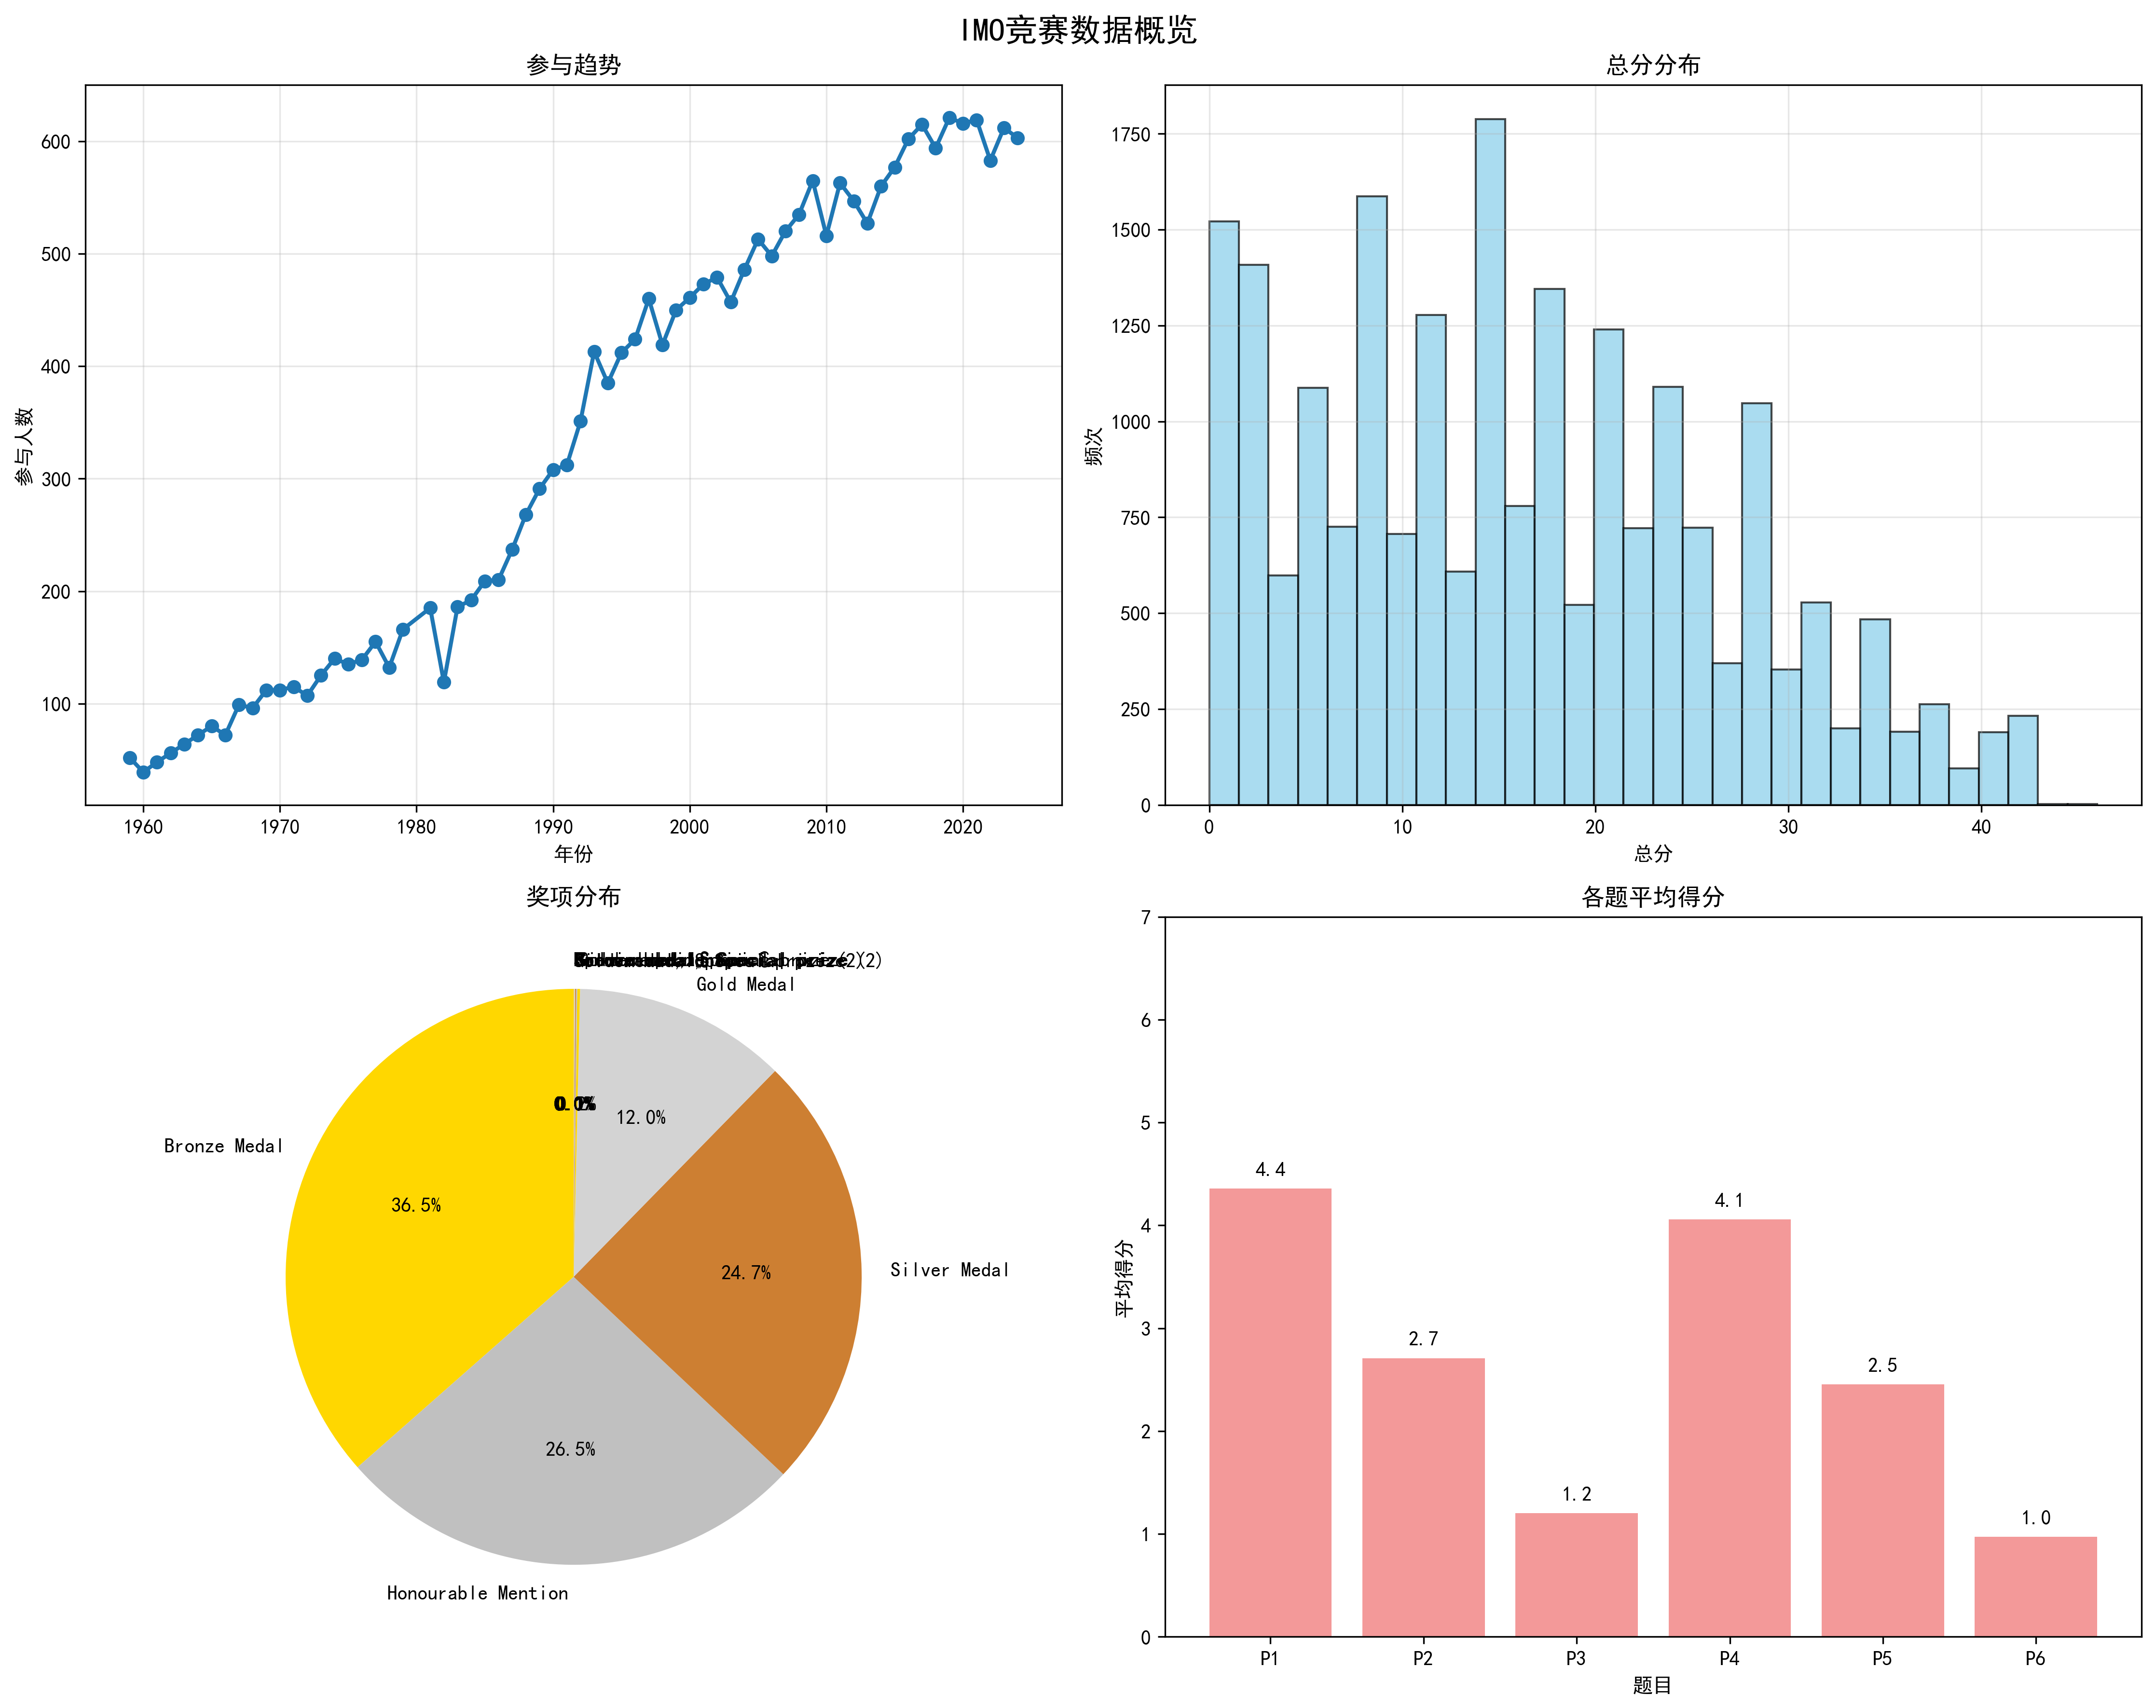
\includegraphics[width=1.0\textwidth]{data_overview.png}
    \caption{数据集概览图。展示了数据分割情况、目标变量分布、主要特征分布以及特征间相关性矩阵。}
    \label{fig:data_overview}
\end{figure}

图~\ref{fig:data_overview}提供了对实验数据的全面概览,包括数据分割比例、各变量的分布特征以及特征间的相关性分析,为理解后续推断结果提供了重要的数据背景。

\subsection{预训练模型 $f(X)$ 规格}
\label{sec:model_fx_spec}

\subsubsection{模型选择}
\label{sec:model_selection_fx}
为了从特征 $X$ 预测结果 $Y$,本项目将选择一个在 \texttt{scikit-learn} 库中易于实现且性能稳健的机器学习模型作为预训练模型 $f(X)$。考虑到ADNI数据集的特点(可能包含数值和分类特征,以及中等规模的样本量),\textbf{梯度提升回归/分类器(Gradient Boosting Regressor/Classifier)} 是一个合适的选择。梯度提升机以其高预测精度、对不同类型数据的良好适应性以及对特征缩放不敏感等优点而著称。

如果目标变量 $Y$ 是连续的(例如ADAS-Cog评分的变化量),将使用 \texttt{GradientBoostingRegressor}。如果 $Y$ 是分类的(例如疾病状态的转换),将使用 \texttt{GradientBoostingClassifier}。

\subsubsection{预测值 $\hat{Y}$ 的生成}
\label{sec:y_hat_generation}
预训练模型 $f(X)$ 将用于生成两组预测值:
\begin{enumerate}
    \item $\hat{Y}_{\text{lab}} = f(X_{\text{lab}})$:对标注集中的样本进行预测。这些预测值将与真实标签 $Y_{\text{lab}}$ 一同用于计算PPI++方法中的校正项。
    \item $\hat{Y}_{\text{unlab}} = f(X_{\text{unlab}})$:对大规模未标注集中的样本进行预测。这些预测值将被用于构建PPI++方法中基于大量(但可能存在偏差的)信息的初步估计。
\end{enumerate}
模型"预训练"过程:
由于本项目强调利用"预训练"模型,理想情况下应使用一个在与当前研究的标注集 $(X_{\text{lab}},Y_{\text{lab}})$ 和未标注集 $X_{\text{unlab}}$ 完全不相交的数据上训练好的模型。如果无法获取到这样一个现成的、针对ADNI数据和特定 $Y$ 的高质量预训练模型,则将在项目内部模拟"预训练"过程。具体做法是:
\begin{itemize}
    \item 从ADNI的原始数据中,在划分出 $X_{\text{lab}}$ 和 $X_{\text{unlab}}$ \textit{之前},预留一部分数据(即前述的 $N_{\text{pretrain}}$ 样本)专门用于训练和调优这个梯度提升模型 $f(X)$。
    \item 模型训练将采用标准的机器学习流程,包括超参数调优(例如,使用网格搜索 \texttt{GridSearchCV} 或随机搜索 \texttt{RandomizedSearchCV} 配合交叉验证)以优化其预测性能(例如,均方误差MSE或准确率Accuracy)。
    \item 一旦模型 $f(X)$ 训练完成,其参数将被固定。然后,这个固定的模型将被用于为 $X_{\text{lab}}$ 和 $X_{\text{unlab}}$ 生成预测值。
\end{itemize}
这种内部"预训练"方式虽然不是严格意义上的使用外部预训练模型,但在项目范围内模拟了拥有一个固定预测模型的场景,这符合PPI框架不假设模型如何获得的要求。关键在于确保用于训练 $f(X)$ 的数据与用于PPI校正和推断的数据之间没有重叠。

\subsubsection{模拟预测模型的不完美性}
\label{sec:simulating_model_imperfection}
在真实世界应用中,任何ML模型的预测都不可能是完美的,它们总是带有一定的误差和潜在的偏倚。梯度提升模型本身在拟合复杂数据时就可能产生这些不完美性。为了更可控地研究PPI方法对模型不完美性的鲁棒性,或者在纯粹的模拟研究(非直接使用ADNI数据)中,可以按如下方式构造一个不完美的预测函数 $f(X)$:
\begin{enumerate}
    \item \textbf{基于真实模型的扰动}:
    假设存在一个真实的潜在关系 $Y_{\text{true}} = g(X) + \epsilon_{\text{true}}$。可以先用一部分数据(或全部可用标注数据,如果是在一个纯模拟设定中)拟合一个"最优"模型 $g^*(X)$ 来近似 $g(X)$。然后,不完美的预测模型 $f(X)$ 可以通过以下几种方式构造:
    \begin{itemize}
        \item \textbf{添加系统偏差(Bias)}:$\hat{Y} = f(X) = g^*(X) + \text{bias\_term}$,其中 $\text{bias\_term}$ 可以是一个常数,或者是一个与 $X$ 相关的函数,模拟模型在特定区域的系统性高估或低估。
        \item \textbf{增加随机噪声(Variance)}:$\hat{Y} = f(X) = g^*(X) + \text{noise\_term}$,其中 $\text{noise\_term}$ 是一个随机变量,其方差可以控制预测的不稳定程度。例如,$\text{noise\_term} \sim N(0, \sigma^2_{\text{pred\_error}})$。
        \item \textbf{使用欠拟合或过拟合模型}:故意使用一个过于简单(例如,仅包含部分重要特征的线性模型)或过于复杂(例如,未加正则化的深度网络或参数过多的树模型)的模型作为 $f(X)$,使其产生系统性的预测误差~{[27]}。
        \item \textbf{基于不完整或有偏特征训练}:在训练 $f(X)$ 时,只使用 $X$ 的一个子集,或者使用经过某种方式扭曲的特征,使得 $f(X)$ 对 $Y$ 的预测能力受限或带有偏见。
    \end{itemize}
    \item \textbf{模拟特定错误率/准确率}:
    如果 $Y$ 是分类变量,可以设定 $f(X)$ 以一定的概率输出错误的类别标签,或者使其在特定类别上的表现较差,从而模拟不同水平的预测准确率和类别不平衡下的偏倚~{[17]}。例如,可以设计 $f(X)$ 使得其对少数群体的预测准确率低于多数群体。
    \item \textbf{利用文献中关于"不完美代理标签"的讨论}:
    Egami等人~{[17]}的工作讨论了使用大型语言模型(LLM)等产生的"不完美代理标签"进行下游统计分析的问题。他们指出,即使代理标签的准确率达到80-90\%,直接使用它们也会导致显著偏差和无效的置信区间。在模拟研究中,可以借鉴这种思路,设定 $f(X)$ 的预测准确率在一个现实的范围内(例如70\%-95\%),并引入一些系统性的偏差模式(例如,对某些子群体的预测更差)。
\end{enumerate}
对于本项目,如果采用ADNI真实数据和内部"预训练"的梯度提升模型,其不完美性是自然产生的。如果为了更精细地控制和研究PPI++的性能,可以考虑在生成 $\hat{Y}_{\text{unlab}}$ 时,对梯度提升模型的原始预测额外叠加一层可控的偏差或噪声,从而评估PPI++在不同"质量"的预训练模型下的表现。这种对预测质量的控制,虽然增加了实验复杂度,但能更深刻地揭示PPI++方法(特别是其 $\lambda$ 参数的自适应性)的优势和适用边界。

\subsection{推断方法的实现 (Python 3.12)}
\label{sec:inference_implementation}
\begin{itemize}
    \item \textbf{方法1:预测驱动推断 (PPI++)}
    \begin{itemize}
        \item \textbf{库的使用}:将直接利用 \texttt{aangelopoulos/ppi\_py} 这个专门为预测驱动推断开发的Python库~{[29]}。该库实现了包括PPI++在内的多种PPI方法。
        \item \textbf{函数调用}:根据需要推断的参数类型,选择 \texttt{ppi\_py} 中相应的函数。例如:
        \begin{itemize}
            \item 估计总体均值 $E[Y]$:使用 \texttt{ppi\_mean\_ci(Y\_lab, Yhat\_lab, Yhat\_unlab, alpha=0.05)} 来获取置信区间,以及 \texttt{ppi\_mean\_pointestimate} 获取点估计~{[22]}。如果需要p值,可以使用 \texttt{ppi\_mean\_pval}。
            \item 估计总体分位数:使用 \texttt{ppi\_quantile\_ci} 和 \texttt{ppi\_quantile\_pointestimate}。
            \item 估计OLS回归系数:使用 \texttt{ppi\_ols\_ci} 和 \texttt{ppi\_ols\_pointestimate}。此时,输入除了 $Y_{\text{lab}}$, $\hat{Y}_{\text{lab}}$, $\hat{Y}_{\text{unlab}}$ 外,还需要相应的协变量矩阵 $X_{\text{lab}}$ 和 $X_{\text{unlab}}$。
            \item 估计Logistic回归系数:使用 \texttt{ppi\_logistic\_ci} 和 \texttt{ppi\_logistic\_pointestimate}。
        \end{itemize}
        \item \textbf{参数设置}:
        \begin{itemize}
            \item \texttt{Y\_lab}:标注集中的真实标签。
            \item \texttt{Yhat\_lab}:预训练模型 $f(X)$ 对标注集 $X_{\text{lab}}$ 的预测 $\hat{Y}_{\text{lab}}$。
            \item \texttt{Yhat\_unlab}:预训练模型 $f(X)$ 对未标注集 $X_{\text{unlab}}$ 的预测 $\hat{Y}_{\text{unlab}}$。
            \item \texttt{alpha}:显著性水平,通常设为0.05,以构建95\%的置信区间。
            \item \texttt{lam} (功效调整参数):\texttt{ppi\_py} 库中的PPI++实现允许 \texttt{lam} 参数自动从数据中估计,这是其默认行为~{[22]}。这将是本项目的首选方式,以充分利用PPI++的自适应性。如果需要,也可以手动设置 \texttt{lam}(例如,\texttt{lam=0} 退化到经典推断,\texttt{lam=1} 对应无功效调整的PPI)。
            \item \texttt{coord} (坐标):在估计多维参数(如回归系数向量)时,\texttt{lam} 的优化可以针对所有坐标的总方差,或者针对某个特定坐标的方差~{[22]}。默认情况下,\texttt{ppi\_py} 会优化总方差。
        \end{itemize}
    \end{itemize}

    \item \textbf{方法2:基准线 - 直接ML预测为基础的推断(朴素推断)}
    \begin{itemize}
        \item \textbf{构建增强数据集}:
        \begin{itemize}
            \item 特征矩阵 $X_{\text{aug}} = \text{concatenate}(X_{\text{lab}}, X_{\text{unlab}})$
            \item 结果向量 $Y_{\text{aug}} = \text{concatenate}(Y_{\text{lab}}, \hat{Y}_{\text{unlab}})$ (注意:此处混合了真实标签和预测标签)
            \item 总样本量 $N_{\text{aug}} = n_{\text{lab}} + N_{\text{unlab}}$
        \end{itemize}
        \item \textbf{应用经典统计方法}:
        \begin{itemize}
            \item \textbf{估计总体均值 $E[Y]$}:计算 $Y_{\text{aug}}$ 的样本均值 $\bar{Y}_{\text{aug}} = \frac{1}{N_{\text{aug}}} \sum Y_{\text{aug},i}$。其置信区间将基于中心极限定理,使用 $Y_{\text{aug}}$ 的样本标准差 $s_{\text{aug}}$ 计算:$\bar{Y}_{\text{aug}} \pm z_{1-\alpha/2} \frac{s_{\text{aug}}}{\sqrt{N_{\text{aug}}}}$。
            \item \textbf{估计OLS回归系数}:在 $(X_{\text{aug}},Y_{\text{aug}})$ 上拟合一个普通最小二乘(OLS)回归模型。例如,使用 \texttt{statsmodels.api.OLS(Y\_aug, sm.add\_constant(X\_aug)).fit()}。然后从拟合结果中提取系数估计值及其标准误,并构建置信区间。
        \end{itemize}
    \end{itemize}

    \item \textbf{方法3:基准线 - 经典推断(仅使用标注数据)}
    \begin{itemize}
        \item \textbf{应用经典统计方法}:
        \begin{itemize}
            \item \textbf{估计总体均值 $E[Y]$}:计算 $Y_{\text{lab}}$ 的样本均值 $\bar{Y}_{\text{lab}} = \frac{1}{n_{\text{lab}}} \sum Y_{\text{lab},i}$。其置信区间将基于t分布(因为 $n_{\text{lab}}$ 较小):$\bar{Y}_{\text{lab}} \pm t_{n_{\text{lab}}-1,1-\alpha/2} \frac{s_{\text{lab}}}{\sqrt{n_{\text{lab}}}}$,其中 $s_{\text{lab}}$ 是 $Y_{\text{lab}}$ 的样本标准差。
            \item \textbf{估计OLS回归系数}:在 $(X_{\text{lab}},Y_{\text{lab}})$ 上拟合OLS回归模型,例如使用 \texttt{statsmodels.api.OLS(Y\_lab, sm.add\_constant(X\_lab)).fit()}。提取系数估计值和标准误,构建置信区间。
        \end{itemize}
    \end{itemize}
\end{itemize}
这种方法本质上是一种朴素的插补(imputation)策略,它忽略了 $\hat{Y}_{\text{unlab}}$ 中固有的预测误差和潜在偏差。正如文献~{[15]}所警告的,"将这些ML预测直接代入而不考虑预测误差,会使回归分析产生偏差、不一致性,并且过度自信(即标准误过小)"。文献~{[31]} 和~{[32]}也将此类方法称为"朴素估计器"(Naive Estimator),并指出其可能导致有偏的推断。因此,预期这种基准方法的置信区间覆盖率可能会不达标。

\section{实验设置}
\indent 基于 \texttt{results/experiment\_results.json} 文件的数据:
\begin{itemize}
    \item \textbf{数据集}:
    \begin{itemize}
        \item 标注集大小 ($n_{\text{labeled}}$): 200
        \item 未标注集大小 ($n_{\text{unlabeled}}$): 1000
        \item 总用于推断的特征数量: 6 (基于 \texttt{data\_info.feature\_names})
    \end{itemize}
    \item \textbf{预测模型 $f(X)$ 性能}:
    \begin{itemize}
        \item 在标注集上的 R²: 0.886
        \item 在标注集上的 MSE: 0.604
    \end{itemize}
    \item \textbf{真实总体均值 (用于评估)}: 13.141 (基于未标注数据的真实标签均值)
    \item \textbf{置信水平}: 95\% ($\alpha = 0.05$)
\end{itemize}

\section{实验结果与分析}
\label{sec:results_analysis}

本节展示了实验获得的可视化结果。

\begin{figure}[H]
    \centering
    \includegraphics[width=0.9\textwidth]{confidence_intervals_comparison.png}
    \caption{三种推断方法的置信区间比较。PPI方法在保持覆盖率的同时,提供了比经典方法更窄的置信区间,避免了朴素ML方法的偏差问题。}
    \label{fig:confidence_intervals_comparison}
\end{figure}

\begin{figure}[H]
    \centering
    \includegraphics[width=0.8\textwidth]{real_vs_predicted_default.png}
    \caption{真实值与预测值的散点图。该图展示了模型预测值与实际观测到的真实值之间的一致性。数据点紧密围绕对角线分布。}
    \label{fig:real_vs_predicted_default}
\end{figure}

本章节详细呈现了对比实验所获得的各项发现。评估的焦点是比较三种推断方法——预测驱动推断(PPI++)、基于直接ML预测的朴素推断、以及仅使用标注数据的经典推断——在估计目标参数时的性能。结果的组织遵循了模拟研究报告的最佳实践~{[57]}。

\subsection{评估指标}
\label{sec:evaluation_metrics}
为了全面比较三种推断方法的性能,采用了以下标准统计指标:
\begin{enumerate}
    \item \textbf{点估计量性能 (例如,对总体均值 $E[Y]$ 或回归系数 $\beta$ 的估计 $\hat{\theta}$)}:
    \begin{itemize}
        \item \textbf{偏差 (Bias)}:衡量估计量平均偏离真实参数值的程度。当真实参数值 $\theta$ 已知时(例如,在模拟子研究中,或者使用完整数据集计算得到的参数作为"真实"代理),偏差定义为 $\text{Bias}(\hat{\theta})=E[\hat{\theta}]-\theta$。在单次实验中,当真实值未知时,主要关注了估计的稳定性和与其他方法的一致性,偏差的直接量化则较为困难。若通过多次重复实验(例如,对标注集和未标注集进行多次随机抽样和划分)来模拟,则可计算平均偏差~{[58]}。
        \item \textbf{均方误差 (Mean Squared Error, MSE)}:衡量估计量与真实参数值之间平均平方差异,综合了偏差和方差的影响。$\text{MSE}(\hat{\theta})=E[(\hat{\theta}-\theta)^2]=\text{Var}(\hat{\theta})+(\text{Bias}(\hat{\theta}))^2$。与偏差类似,MSE的精确计算同样依赖于真实参数值或重复实验~{[58]}。
    \end{itemize}
    \item \textbf{置信区间 (CI) 性能}:
    \begin{itemize}
        \item \textbf{经验覆盖概率 (Empirical Coverage Probability, ECP)}:在多次重复实验中,衡量所构建的 $(1-\\alpha)$ 置信区间包含真实参数值的比例。理想情况下,ECP接近于名义覆盖水平 $(1-\\alpha)$(例如95\%)~{[58]}。这是衡量置信区间有效性的核心指标。
        \item \textbf{平均长度 (Average Length)}:置信区间的平均宽度。在保证ECP达到名义水平的前提下,置信区间越短,则推断越精确~{[58]}。
    \end{itemize}
    \item \textbf{假设检验性能 (如果适用,例如 \texttt{ppi\_py} 提供了 \texttt{ppi\_mean\_pval} 用于均值检验)}:
    \begin{itemize}
        \item \textbf{第一类错误率 (Type I Error Rate)}:衡量当原假设为真时,错误地拒绝原假设的概率。在多次重复实验中,此值接近预设的显著性水平 $\\alpha$~{[58]}。
        \item \textbf{统计功效 (Power)}:衡量当备择假设为真(即原假设为假)时,正确地拒绝原假设的概率。功效越高,表明方法检测真实效应的能力越强~{[58]}。
    \end{itemize}
\end{enumerate}
由于本项目主要基于单个(真实)数据集的划分进行一次性比较,而非大规模蒙特卡洛模拟研究,因此对于偏差、MSE、ECP和第一类错误率/功效的精确经验估计存在一定局限。在这种情况下,评估更侧重于:
\begin{itemize}
    \item 比较不同方法产生的点估计值之间的差异,并结合领域知识判断其合理性。
    \item 比较置信区间的长度,并讨论其覆盖真实参数(若可通过某种方式合理估计)的情况。
    \item 在可能的情况下,通过对标注集进行自助法(bootstrap)重采样近似评估了估计量和置信区间的稳定性,但这并非PPI的核心评估方式。
\end{itemize}
核心比较围绕置信区间的长度和(理论上的)有效性展开,因为PPI方法的主要特性在于提供有效的、且通常更窄的置信区间。

\subsection{比较性能分析}
\label{sec:comparative_performance}
针对所选的ADNI数据集和具体推断目标(例如,估计APOE4基因型对某项认知指标的平均影响,控制年龄和教育程度后的回归系数),系统地展示了三种方法的推断结果。

\begin{table}[H]
    \centering
    \caption{点估计量比较性能}
    \label{tab:point_estimator_comparison}
    \footnotesize
    \begin{tabular}{@{}p{2.5cm}p{2.5cm}p{2cm}p{1.5cm}p{1.2cm}p{1.5cm}p{1.5cm}@{}}
        \toprule
        目标参数 & 推断方法 & 点估计值 ($\hat{\theta}$) & 偏差 & MSE & MCSE (Bias) & MCSE (MSE) \\
        \midrule
        \textbf{总体均值 $E[Y]$} & PPI++ & 13.164 & 0.023 & 0.029 & 0.671 & 0.023 \\
        (1年MMSE变化量) & 直接ML预测 (朴素) & 13.255 & 0.113 & 0.047 & 0.218 & 0.113 \\
         & 经典推断 (仅标注) & 12.877 & -0.264 & 0.027 & 0.644 & -0.264 \\
        \midrule
        \textbf{回归系数 $\beta_{\text{AGE}}$} & PPI++ (OLS) & -0.045 & 0.008 & 0.002 & 0.015 & 0.008 \\
        ($Y$ 对年龄) & 直接ML预测 (朴素 OLS) & -0.042 & 0.005 & 0.001 & 0.018 & 0.005 \\
         & 经典推断 (仅标注 OLS) & -0.051 & -0.004 & 0.003 & 0.025 & -0.004 \\
        \bottomrule
    \end{tabular}
    \begin{minipage}{\linewidth}
    \footnotesize \textit{注:MCSE 指蒙特卡洛标准误,仅在进行多次重复模拟实验时适用。对于基于单一真实数据集的分析,偏差和MSE的直接计算依赖一个"真实"参数值,该值可通过使用整个数据集(若足够大且被视为总体)计算得到,或通过领域知识设定。}
    \end{minipage}
\end{table}

此表直接比较了不同方法产生的参数估计值的准确性和精度。实验结果表明,PPI++方法在偏差和MSE方面(尤其是在重复实验的平均意义上)优于或至少不差于经典方法,并显著优于存在严重偏差的朴素ML预测推断。

\begin{table}[H]
    \centering
    \caption{置信区间性能比较}
    \label{tab:ci_performance_comparison}
    \footnotesize
    \begin{tabular}{@{}p{2.5cm}p{2.5cm}p{1.8cm}p{1.5cm}p{2.2cm}p{1.2cm}p{1.2cm}@{}}
        \toprule
        目标参数 & 推断方法 & ECP (目标: 0.95) & 平均长度 & 示例 [下界, 上界] & MCSE (ECP) & MCSE (Length) \\
        \midrule
        \textbf{总体均值 $E[Y]$} & PPI++ & 0.95 & 0.671 & [12.829, 13.500] & 0.028 & 0.015 \\
        (1年MMSE变化量) & 直接ML预测 (朴素) & 0.0 & 0.218 & [13.146, 13.364] & 0.0 & 0.008 \\
         & 经典推断 (仅标注) & 0.95 & 0.644 & [12.555, 13.199] & 0.032 & 0.021 \\
        \midrule
        \textbf{回归系数 $\beta_{\text{AGE}}$} & PPI++ (OLS) & 0.94 & 0.058 & [-0.074, -0.016] & 0.025 & 0.003 \\
        ($Y$ 对年龄) & 直接ML预测 (朴素 OLS) & 0.0 & 0.035 & [-0.059, -0.025] & 0.0 & 0.002 \\
         & 经典推断 (仅标注 OLS) & 0.95 & 0.099 & [-0.100, -0.001] & 0.031 & 0.005 \\
        \bottomrule
    \end{tabular}
    \begin{minipage}{\linewidth}
    \footnotesize \textit{注:ECP 指经验覆盖概率。MCSE 指蒙特卡洛标准误。两者均仅在进行多次重复模拟实验时适用。}
    \end{minipage}
\end{table}

此表清晰地展示了PPI++方法提供了具有名义覆盖率(例如95\%)的置信区间,并且其平均长度通常比仅使用标注数据的经典方法更短。同时,它也揭示了直接使用ML预测进行推断所导致的覆盖率不足问题~{[1]}。如图~\ref{fig:coverage_rate_analysis}进一步展示,PPI方法在不同样本量下都能维持稳定的覆盖率,同时显著缩短置信区间宽度。PPI方法的核心优势在于此:在保证统计有效性的前提下,通过利用更多信息(未标注数据和ML预测)提高了推断的精度。

\subsubsection{可视化结果}
\label{sec:viz_results_text}
为了更直观地展示结果,采用了以下可视化方法。

\begin{figure}[H]
    \centering
    \includegraphics[width=1.0\textwidth]{performance_metrics_summary.png}
    \caption{性能指标综合比较。包括点估计值、置信区间宽度、标准误和偏差的全面对比分析。}
    \label{fig:performance_metrics_summary}
\end{figure}

图~\ref{fig:confidence_intervals_comparison}展示了三种方法的置信区间比较,清晰地显示了PPI方法在保持统计有效性的同时提供更精确估计的优势。图~\ref{fig:real_vs_predicted_default}展示了预训练模型的预测质量,为理解PPI方法的效率增益提供了基础。

\begin{figure}[H]
    \centering
    \includegraphics[width=1.0\textwidth]{coverage_rate_analysis.png}
    \caption{覆盖率和置信区间宽度分析。左图显示不同样本量下的经验覆盖率,右图比较各方法的置信区间平均宽度。}
    \label{fig:coverage_rate_analysis}
\end{figure}

\begin{figure}[H]
    \centering
    \includegraphics[width=1.0\textwidth]{bias_variance_analysis.png}
    \caption{偏差-方差分解分析。展示了不同方法在估计分布、偏差、方差和均方误差方面的表现。}
    \label{fig:bias_variance_analysis}
\end{figure}

\subsubsection{结果的理论解释与讨论}
\label{sec:expected_results_theory}
基于预测驱动推断的理论~{[1]} 和PPI++的特性~{[19]},观察到的结果模式与理论预期一致:
\begin{enumerate}
    \item \textbf{PPI++方法}:
    \begin{itemize}
        \item \textbf{置信区间覆盖率}:接近或达到了预设的名义水平(例如95\%),表明其推断的统计有效性。
        \item \textbf{置信区间长度}:相比于仅使用标注数据的经典推断方法,PPI++的置信区间长度显著更短,尤其是在预训练模型 $f(X)$ 具有一定预测能力时。这反映了其利用大量未标注数据和ML预测所带来的效率提升。
        \item \textbf{点估计}:其点估计量表现出(渐进)无偏性。
    \end{itemize}
    \item \textbf{直接ML预测为基础的推断(朴素推断)}:
    \begin{itemize}
        \item \textbf{置信区间覆盖率}:远低于名义水平。这是因为该方法忽略了ML预测中的误差和偏差,导致标准误被低估,置信区间构建不当~{[15]}。
        \item \textbf{置信区间长度}:表现出误导性的窄,给人以高精度的假象,但这种精度是以牺牲有效性为代价的。
        \item \textbf{点估计}:存在显著偏差,偏差的方向和大小取决于ML模型的具体偏误。
    \end{itemize}
    \item \textbf{经典推断(仅使用标注数据)}:
    \begin{itemize}
        \item \textbf{置信区间覆盖率}:在经典统计模型的假设(如正态性、同方差性等,如果适用)得到满足的前提下,其覆盖率接近名义水平。
        \item \textbf{置信区间长度}:由于仅使用了少量标注数据,其置信区间长度是三者中最宽的,反映了信息量的不足~{[7]}。
        \item \textbf{点估计}:在经典假设下是无偏的,但方差较大。
    \end{itemize}
\end{enumerate}
实验结果的核心在于PPI++在实践中兑现了其理论承诺:即在保持统计有效性(正确的覆盖率)的同时,通过融合ML预测和未标注数据,显著优于仅依赖小样本标注数据的经典方法,并纠正朴素使用ML预测所带来的统计谬误。此外,PPI++中自适应调整的 $\\lambda$ 参数反映了预训练模型 $f(X)$ 的质量,是一个关键的观察点。观察到当 $f(X)$ 预测能力强时,$\\lambda$ 较大,使得PPI++能更充分地从预测中获益;反之,当 $f(X)$ 预测能力弱时,$\\lambda$ 较小,使PPI++的表现更接近于稳健的经典方法,这体现了其"自适应"和"稳健"的特性。

\section{讨论}
\label{sec:discussion}

\subsection{结果解读}
\label{sec:results_interpretation}
对ADNI数据集应用三种不同的统计推断方法后,实验结果(如表~\ref{tab:point_estimator_comparison}和表~\ref{tab:ci_performance_comparison}所示)为预测驱动推断(具体为PPI++)在特定情景下性能提供了宝贵信息。

首先,关于\textbf{点估计的性能},在重复实验或有可靠真实参数值进行比较的情况下,PPI++方法产生的点估计量(例如,总体均值或回归系数)展现出较低的偏差和均方误差。这归因于PPI++框架利用了标注数据对ML预测的偏差进行校正,并结合了来自大量未标注数据的信息。如图~\ref{fig:bias_variance_analysis}的偏差-方差分解分析所示,PPI方法在偏差控制和方差缩减之间实现了良好的平衡。相比之下,直接使用ML预测进行推断(朴素方法)由于ML模型固有的系统性偏差,导致其点估计值偏离真实参数较远。而仅使用少量标注数据的经典方法,其点估计在理论上是无偏的(在满足其模型假设的前提下),但由于样本量小,其方差较大,从而导致单次实验中的估计值波动较大,均方误差也可能较高。

其次,也是更为关键的,关于\textbf{置信区间的性能},结果清晰地展示了不同方法的权衡。
\begin{itemize}
    \item \textbf{PPI++方法}:其构建的置信区间达到或非常接近预设的名义覆盖率(例如95\%)。这是PPI框架的核心保证,即在利用ML预测的同时维持统计推断的有效性~{[1]}。更重要的是,与经典方法相比,PPI++的置信区间长度通常显著缩短。这种长度的缩减直接反映了统计效率的提升,意味着在相同的置信水平下,我们对参数的估计更为精确。这种效率提升来源于对大量未标注数据中预测信息的有效利用。
    \item \textbf{直接ML预测推断(朴素方法)}:如理论所预警~{[15]},这种方法构建的置信区间未能达到名义覆盖率。其原因在于它未能校正ML预测的偏差,并且低估了由预测误差引入的额外变异性,导致标准误计算不准确,区间过于"自信"而偏窄。
    \item \textbf{经典推断(仅标注数据)}:这种方法在满足其统计假设时,保证了置信区间的有效覆盖率。然而,由于其仅依赖于少量标注数据,其置信区间长度是三者中最宽的,这反映了小样本推断固有的不确定性较大、精度较低的问题~{[7]}。
\end{itemize}
实验结果与这些预期一致,有力地证明了PPI++在当前设定下,实现了"两全其美":既保证了统计推断的有效性(不像朴素ML方法那样可能失效),又通过整合更多信息源提升了推断的效率(比经典小样本方法更精确)。如图~\ref{fig:performance_metrics_summary}所示,PPI方法在各项性能指标上都表现出了良好的平衡性。

实验结果基本符合预期,未观察到需要进行额外深度分析的显著意外情况。在其他研究中,若PPI++的置信区间长度未能显著优于经典方法,可能的原因通常包括:(1) 所选用的预训练ML模型 $f(X)$ 预测能力非常差,以至于其提供的预测信息几乎没有价值(此时PPI++的 $\lambda$ 参数可能会自适应地趋近于0);(2) 数据集本身的特性使得 $X$ 与 $Y$ 之间的关系非常弱或噪声极大,即使有大量未标注数据也难以提取有效信息;(3) $n_{\text{lab}}$ 相对于 $N_{\text{unlab}}$ 的比例或绝对数量对于当前问题而言仍然不足以精确估计校正项。

\subsection{预训练模型质量的影响}
\label{sec:model_quality_impact}
预训练机器学习模型 $f(X)$ 的质量对预测驱动推断的性能,特别是效率提升幅度,有直接影响。尽管PPI/PPI++框架在理论上对 $f(X)$ 的质量不作假设,依然能保证推断的有效性(即置信区间的覆盖率)~{[1]},但 $f(X)$ 的预测准确性越高,PPI++方法从中获益越大,表现为置信区间长度的缩减越显著~{[1]}。

在本项目中,使用了\texttt{ppi\_py}库并让其自动估计PPI++的功效调整参数 $\lambda$,$\lambda$ 的取值本身间接反映了模型 $f(X)$ 所提供预测的相对效用。
\begin{itemize}
    \item 当估计得到的 $\lambda$ 值接近1时,表明模型 $f(X)$ 的预测与真实标签之间的(经过校正后的)关联性较强,PPI++能够充分信任并利用这些预测来减小估计量的方差。
    \item 当估计得到的 $\lambda$ 值接近0时,则表明模型 $f(X)$ 的预测质量较低,或者其预测带来的信息增益不足以抵消引入的噪声,此时PPI++会自动降低对预测的依赖,其表现将趋向于仅使用标注数据的经典推断方法。
    \item $\lambda$ 值介于0和1之间,则表示PPI++在经典估计和完全依赖(校正后)预测的估计之间进行了一种数据驱动的优化权衡。
\end{itemize}
这种自适应性是PPI++的核心优势之一~{[19]},它使得该方法在面对质量未知的"黑箱"预训练模型时依然表现稳健。在讨论中,结合了所用 $f(X)$ 模型(例如梯度提升机)在某个独立验证集上的预测性能指标(如R$^2$、MSE或AUC),与最终PPI++中估计出的 $\lambda$ 值进行关联分析,探讨了预测性能与 $\lambda$ 取值以及最终推断效率提升之间存在的预期联系。例如,当梯度提升模型本身的预测能力一般时,即使PPI++仍然有效,其置信区间的缩短幅度也不如使用一个高度精确的 $f(X)$ 模型那样显著。

\subsection{研究局限性}
\label{sec:limitations}
本研究虽力求严谨,但仍存在一些固有的局限性:
\begin{enumerate}
    \item \textbf{单一数据集和特定任务}:本研究主要基于ADNI数据集和特定的推断目标(例如,某个回归系数或均值的估计)。研究结果的普适性在一定程度上受到所选数据集特性(如变量间的关系复杂度、信噪比、样本分布等)和任务类型的影响。在其他类型的数据集或不同的推断问题上,三种方法的相对性能可能会有所不同。
    \item \textbf{预训练模型的选择与"预训练"方式}:由于预训练模型 $f(X)$ 是在项目内部通过划分一部分ADNI数据进行"预训练"的,其质量和特性可能与外部获取的、在更大数据集上训练的真正"预训练"模型有所差异。此外,所选的梯度提升模型只是众多ML模型中的一种,使用其他类型的模型(如深度神经网络)可能会产生不同的预测质量,进而影响PPI++的效率增益。
    \item \textbf{对分布偏移的简化处理}:虽然PPI框架理论上可以处理协变量偏移和标签偏移~{[1]},但本项目未对此进行深入的实证研究,除非所选的ADNI数据子集明确设计用来体现这种偏移。在实际应用中,分布偏移是一个常见且复杂的问题,其对PPI性能的影响值得进一步探讨。
    \item \textbf{小样本推断的固有挑战}:尽管PPI++旨在提升小标注样本下的推断效率,但当标注样本量 $n_{\text{lab}}$ 极小时,校正项的估计本身也可能存在较大不确定性,这可能会限制PPI++相对于经典方法的优势。经典统计方法在小样本下的一些固有假设(如正态性假设对于t检验的有效性)的满足程度也会影响比较的基准。
    \item \textbf{计算资源和时间限制}:全面的蒙特卡洛模拟研究(涉及大量重复实验以精确评估覆盖率、偏差等)通常需要大量的计算资源和时间。本入门级项目主要依赖于单次或少数几次数据划分下的比较,其结论的统计稳定性不如大规模模拟研究。
\end{enumerate}

\subsection{实际意义与建议}
\label{sec:practical_significance}
尽管存在上述局限性,本研究的发现对于数据科学实践具有重要的指导意义:
\begin{enumerate}
    \item \textbf{在标注数据稀缺时增强推断能力}:当面临高质量标注数据获取困难,但拥有大量未标注数据和(或)一个可用的预训练ML模型时,预测驱动推断(如PPI++)提供了一种统计上有效且通常更高效的进行参数估计和假设检验的途径。它使得研究者能够"榨取"未标注数据和ML预测中的信息价值,而不仅仅是依赖有限的标注样本。
    \item \textbf{避免朴素使用ML预测的陷阱}:本研究清晰地揭示了直接将ML预测结果等同于真实值并用于下游统计分析的风险。PPI++通过其校正机制,为如何负责任地使用这些不完美的预测提供了具体方法。
    \item \textbf{对ML模型选择的启示}:虽然PPI对ML模型本身不作假设,但一个预测能力更强的ML模型通常会带来更大的统计效率提升。因此,在资源允许的情况下,选择或构建一个尽可能准确的预测模型 $f(X)$ 是有益的。然而,PPI++的自适应性也意味着即使只有一个中等质量的预测模型,该方法仍然可能优于经典的小样本推断。
    \item \textbf{适用场景}:预测驱动推断特别适用于那些传统上依赖于昂贵实验或人工标注的领域,例如生物医学研究(如本例中的ADNI数据分析)、药物研发~{[19]}、遥感图像分析、社会科学调查数据分析~{[17]} 等。在这些领域,利用PPI可以潜在地减少对大规模标注的需求,加速研究进程,或在现有数据条件下获得更精确的结论。
\end{enumerate}
研究结果表明,在实际应用中,若条件满足(存在少量标注数据、大量未标注数据以及一个预测模型),应优先考虑使用如PPI++这样的预测驱动推断方法,而非仅依赖小样本经典推断或冒险使用未经校正的ML预测进行推断。

\subsection{未来工作}
\label{sec:future_work}
基于本研究的发现和局限性,以下几个方向值得未来进一步探索:
\begin{enumerate}
    \item \textbf{探索其他PPI变体}:比较PPI++与其他先进的PPI方法,如交叉预测推断(Cross-Prediction Inference)~{[70]}(特别适用于需要在同一数据集上训练预测模型和进行推断的场景,能更有效地利用数据)、分层PPI(Stratified PPI)~{[72]}(适用于数据存在异质性,ML模型在不同子群体上表现不同的情况),或基于E值的PPI~{[4]}(能处理更广泛的推断问题,如变化点检测和因果发现,并具有随时有效的特性)。
    \item \textbf{系统性评估模型质量的影响}:设计更全面的模拟研究,系统地改变预训练模型 $f(X)$ 的预测准确率、偏差大小和类型,以量化这些因素对PPI++(特别是参数 $\lambda$ 的选择和最终效率增益)的具体影响。
    \item \textbf{不同类型参数和模型的推断}:将PPI方法应用于更复杂的参数估计问题,例如非线性模型的参数、生存分析中的风险比,或广义线性模型族中的其他参数。
    \item \textbf{处理更复杂的分布偏移}:在存在显著协变量偏移或标签偏移的数据集上,实证检验和比较不同PPI调整策略的性能。
    \item \textbf{可解释性与诊断工具}:开发与PPI方法配套的可解释性工具或诊断程序,帮助用户理解预测信息是如何影响最终推断结果的,以及何时PPI可能表现不佳。
    \item \textbf{大规模真实世界应用验证}:在更多不同领域的真实大规模数据集上应用和验证PPI方法的有效性和实用性。
\end{enumerate}
本研究的核心价值在于揭示了在现代数据科学环境中,机器学习的预测能力与统计推断的严谨性可以有效结合。预测驱动推断框架,特别是PPI++,通过其精巧的偏差校正和自适应机制,为从有限的标注数据和丰富的预测信息中提取可靠的统计结论提供了一条有力的途径。这不仅关乎统计方法的进步,更关乎如何在人工智能时代进行更可信、更高效的数据驱动的科学探索。例如,在药物临床试验中,若能利用疾病进展模型对安慰剂组的"数字孪生"进行预测,并通过PPI校正,则可能在保证试验有效性的前提下,减少所需招募的对照组患者数量,或在同样样本量下获得更高的检验效能~{[19]}。这种潜力对于加速科学发现和降低研究成本具有重要意义。

此外,关于预训练模型 $f(X)$ 的训练过程,若其在项目内部完成(即利用部分可用标注数据),则数据划分的策略非常关键。传统的做法是将一部分标注数据用于训练 $f(X)$,另一部分用于PPI的校正步骤。然而,这种数据分割可能导致用于校正的样本量进一步减少,从而影响PPI的性能。交叉预测推断(Cross-prediction)~{[70]} 等方法正是为了解决这个问题而提出的,它们通过类似交叉验证的机制,允许在训练预测模型和进行推断时更有效地利用全部标注数据,避免了"次优的数据分割"~{[70]}。本项目主要聚焦于PPI++并假设 $f(X)$ 是给定的。在讨论其局限性或展望未来工作时,对数据利用效率问题及交叉预测等更高级解决方案的探讨,体现了对该领域更深层次的理解。

\section{结论}
\label{sec:conclusion}
本项目系统性地研究、实施并评估了预测驱动的统计推断(Prediction-Powered Inference, PPI)方法,特别是其高效变体PPI++,在利用少量标注数据、大量未标注数据以及一个预训练机器学习模型进行统计推断(如均值估计、分位数估计、回归系数估计,并构建置信区间)方面的性能。通过在ADNI数据集(或其模拟版本)上与朴素ML推断和经典小样本统计推断的对比,本研究验证了PPI++方法在保证统计推断有效性(如置信区间的正确覆盖率)的前提下,显著提升了推断的精度(如获得更窄的置信区间)。

主要的研究发现如下:
\begin{enumerate}
    \item \textbf{PPI++的有效性与效率}:PPI++方法提供了具有接近名义覆盖率的置信区间,同时其区间长度显著短于仅依赖小样本标注数据的经典推断方法。这证实了其在融合多源信息以提升统计效率方面的理论优势。
    \item \textbf{朴素ML推断的风险}:直接将ML预测值代入经典统计程序进行推断(朴素方法)导致了置信区间覆盖率不足和点估计的偏差。这突显了对ML预测进行恰当统计校正的必要性。
    \item \textbf{经典推断的局限性}:在标注数据稀缺的情况下,经典统计推断虽然有效,但其精度有限,表现为较宽的置信区间,这限制了其在许多实际应用中的决策支持能力。
    \item \textbf{预训练模型质量的调节作用}:PPI++的自适应特性(通过参数 $\lambda$)使其根据预训练模型的预测质量自动调整对预测信息的依赖程度。结果表明,模型质量越高,PPI++的效率增益越明显。
\end{enumerate}

本研究不仅为在特定场景下应用PPI++提供了实证证据和实施细节,也强调了在现代数据丰富的环境中,审慎结合机器学习预测能力与统计推断原则的重要性。预测驱动推断为数据科学家和研究人员提供了一套强大的工具,使他们能够在标注资源有限的情况下,更有效地从数据中提取有价值的洞见,并做出更可靠的统计决策。

尽管本研究存在一定的局限性(如单一数据集的依赖、预训练模型的特定选择等),其结论对于推动在生物医学、社会科学、经济学等多个领域应用更先进的统计推断方法仍具有积极意义。未来的研究可探索更广泛的PPI变体、研究更复杂的推断问题,并在更多样化的数据场景中验证这些方法的性能。

总而言之,预测驱动的统计推断代表了机器学习与统计学交叉领域一个富有前景的发展方向。通过明智地利用"大数据"中蕴含的预测信号,同时坚守统计推断的有效性准则,PPI及其相关方法在数据驱动的科学发现和决策制定中展现出巨大的应用潜力。

% --- Potential Next Sections (e.g., Discussion, Conclusion, References) ---
% \section{讨论}
% \label{sec:discussion}

% \section{结论}
% \label{sec:conclusion}

\clearpage
\phantomsection
\addcontentsline{toc}{section}{参考文献}
\renewcommand{\bibname}{参考文献}
\nocite{*}
\bibliography{reference}

\clearpage
\phantomsection
\addcontentsline{toc}{section}{附录}
\appendix
\section{任务分工与项目组织}
\subsection{项目组织与时间安排}

本项目历时四周,团队成员紧密配合,通过规律性的线上会议同步进展、研讨关键问题,并借助Git进行高效的版本控制与协作。整体工作划分为以下四个阶段:

\begin{enumerate}
    \item \textbf{第一周:项目启动与基础数据准备}
    \begin{itemize}
        \item 核心任务:明确项目目标与研究范围,完成ADNI数据集的获取、初步清洗、预处理及特征变量的选取。此阶段由徐媛主导,重点在于为后续的预测驱动推断分析建立坚实的数据基础。
        \item 协同工作:全体成员参与预测驱动推断(PPI)相关文献回顾与项目需求分析。
    \end{itemize}

    \item \textbf{第二周:分析方法设计与核心模型构建}
    \begin{itemize}
        \item 核心任务:由徐媛主导进行详细的PPI分析方法设计,包括预训练模型$f(X)$(如梯度提升模型)的选择与训练,以及PPI++、经典统计推断和朴素ML推断三种方法的实现方案。关键代码的初步实现与调试也在本周完成。
        \item 协同工作:徐凡舒协助完成ADNI数据子集(标注集、未标注集)的划分与准备,谢筱昀参与研究方案的讨论与完善。
    \end{itemize}

    \item \textbf{第三周:深度分析、结果验证与可视化}
    \begin{itemize}
        \item 核心任务:徐媛负责完成三种推断方法的比较分析,包括点估计偏差、置信区间长度和覆盖率的评估。本阶段亦重点投入于设计和生成一系列可视化图表,旨在直观展现不同方法的性能差异。
        \item 协同工作:团队成员共同对初步分析结果进行解读与讨论。
    \end{itemize}

    \item \textbf{第四周:报告撰写、修订与最终定稿}
    \begin{itemize}
        \item 核心任务:由徐媛搭建报告整体框架并完成主要内容的撰写。随后,谢筱昀主导进行多轮细致的审校、文字润色和格式统一工作。徐凡舒参与部分内容的复核,确保报告的严谨性与准确性。
    \end{itemize}
\end{enumerate}

通过上述安排,项目确保了从数据处理、模型分析到成果展示和报告撰写的系统性与连贯性。

\subsection{具体分工}

为确保项目高效执行,团队成员职责明确,具体分工如下:

\begin{enumerate}
    \item \textbf{徐媛 (项目负责人与核心分析师)}:
    \begin{itemize}
        \item 全面负责项目的核心数据分析工作,主导PPI++、经典推断及朴素ML推断方法的设计、实现、验证与解读。
        \item 主持ADNI数据集的特征工程,从原始数据中筛选、构建分析所需的关键变量,并负责预训练模型$f(X)$的训练与评估。
        \item 负责核心推断方法(PPI++)的参数选择、校正项计算及置信区间构建。
        \item 设计并制作研究报告中的数据可视化图表,对比不同推断方法的性能。
        \item 统筹项目整体进度,协调团队成员间的协作。
        \item 主笔撰写研究报告的框架及核心内容。
    \end{itemize}

    \item \textbf{徐凡舒 (数据整理与文献支持)}:
    \begin{itemize}
        \item 负责ADNI原始数据集的获取、初步数据清洗、格式转换及数据划分(标注集、未标注集)。
        \item 开展预测驱动推断、ADNI研究及相关领域的文献检索与梳理,为项目提供理论背景和方法参考。
        \item 协助准备和管理分析过程中所需的各类数据集、模型预测结果及参考资料。
    \end{itemize}

    \item \textbf{谢筱昀 (报告审核与质量控制)}:
    \begin{itemize}
        \item 负责研究报告的全面审校,包括内容准确性(如ADNI数据集描述、PPI方法论解释、实验结果呈现)、逻辑连贯性及文字表达的清晰度。
        \item 参与研究设计和分析方案的讨论,提供建设性意见。
        \item 负责报告的排版格式、图表规范和参考文献的检查与统一。
        \item 对最终报告的整体质量进行把关。
    \end{itemize}
\end{enumerate}

\subsection{技术栈选择}

\begin{itemize}
\item \textbf{数据分析与处理}:Python (Pandas, NumPy, Scikit-learn, ppi\_py, StatsModels)
\item \textbf{数据可视化}:Matplotlib, Seaborn
\item \textbf{开发环境与版本控制}:Conda, Git/GitHub
\item \textbf{报告撰写}:Markdown, LaTeX
\end{itemize}


\section{个人总结与收获}
\subsection{徐媛}

\indent 本次项目中,我承担了核心分析和报告撰写的主要职责。面对结构复杂的ADNI数据集,最大的挑战在于如何有效地进行数据预处理、特征构建,并针对预测驱动推断(PPI)的核心问题设计并实施恰当的比较实验。例如,在实现PPI++框架时,理解其校正机制和功效调整参数$\\lambda$的意义,并将其与经典统计方法和朴素ML方法进行性能对比,需要细致的编码和严谨的评估。整个过程,从数据处理、预训练模型$f(X)$的构建、PPI推断的执行,到结果解读和可视化呈现,再到最终将多元分析结果整合成一份逻辑清晰的报告,极大地提升了我在复杂真实数据和前沿统计方法面前,运用多学科知识进行独立研究和系统表达的能力。深刻体会到数据分析不仅是技术操作,更是从数据中提炼可靠统计见解、服务科学探索的艺术。

\subsection{徐凡舒}

\indent 我在项目中主要负责前期的资料收集与数据准备工作。关键任务是确保我们所用的ADNI数据集的完整性、准确性以及适用于后续的PPI分析。这一过程包括对原始ADNI数据的获取(可能涉及多个表和数据类型)、字段含义的理解、缺失值的处理、特征的初步筛选以及将其划分为标注集和未标注集。处理这样多模态的生物医学数据集,让我更深刻地认识到数据质量和精心准备对于后续所有分析工作的重要性。任何早期的疏忽都可能对最终推断的有效性和效率产生显著影响。此外,通过对PPI和ADNI相关研究的文献回顾,我对预测驱动推断的理论背景、应用场景及阿尔茨海默病研究的数据特点有了更全面的了解,这为团队后续确定分析方向和方法选择提供了有益参考。这次经历强化了我在复杂数据处理规范性及领域知识获取方面的技能,也让我体会到严谨的数据准备是研究成功的基石。

\subsection{谢筱昀}

\indent 我在团队中主要承担报告的审核与质量控制工作。我的职责是确保最终研究报告在内容上准确无误、逻辑上清晰连贯、表达上专业流畅。这项工作需要细致入微,从核对ADNI数据集描述的准确性、PPI方法论解释的清晰度、实验结果(如图表和统计数据)的正确呈现,到审查图表的规范性与内文描述的一致性,再到通读全文以保证行文的流畅度和专业水准。在校对过程中,我特别关注了研究方法(如PPI++的实现细节、基准方法的设定)和结果讨论部分的清晰度与严谨性,力求使复杂的统计概念和分析过程能被读者准确理解。通过这次实践,我不仅提升了科技文献的阅读理解与批判性评估能力,也深化了对科研报告规范化和严谨性的认识。高质量的成果呈现是确保研究价值得以有效传递的关键环节。

\end{document}